\documentclass[12pt,a4paper,oneside]{report}
\usepackage[left=2.50cm, right=2.50cm, top=2.50cm, bottom=2.50cm]{geometry}
\usepackage{amsmath, amsfonts, amsthm, amssymb}
\usepackage[utf8]{inputenc}
\usepackage[english]{babel}
\usepackage[backend=biber,style=numeric]{biblatex}
\usepackage[draft, danish]{fixme}

\usepackage{graphicx}
\usepackage{siunitx}
\usepackage{caption}
\usepackage{float}
\usepackage{enumitem}
\usepackage{minted}
\usepackage{showexpl}
\usepackage{url,textcomp}
\usepackage[hidelinks]{hyperref}
\usepackage{cleveref}
\usepackage{pdfpages}

\usepackage{subfig}
\usepackage{wrapfig}

\usepackage{tabularx, multirow, booktabs}
\usepackage{threeparttable}
\usepackage{longtable, tabu}

\usepackage{titlesec}
\usepackage[numbered,breaklines=true]{mcode}

\addbibresource{references.bib} 

%-----------------------------------------------------------------
%   HEADER SECTION
%-----------------------------------------------------------------
\usepackage{fancyhdr}
\pagestyle{fancy}
\fancyhf{}
\rhead{Exam Project}
\lhead{ITAMS}
\rfoot{\thepage}


\author{Jonas Lind; Emil Jepsen}
\title{Applied Microcontroller Systems}
\begin{document}

%-----------------------------------------------------------------
%   TITLE SECTION
%-----------------------------------------------------------------
\begin{titlepage}
	\centering
	{\scshape\LARGE Applied Microcontroller Systems \par}
	\vspace{1cm}
	{\scshape\Large Exam Project\par}
	\vspace{1.5cm}
	{\huge\bfseries Counting Scale \par}
	\vspace{.8cm}
	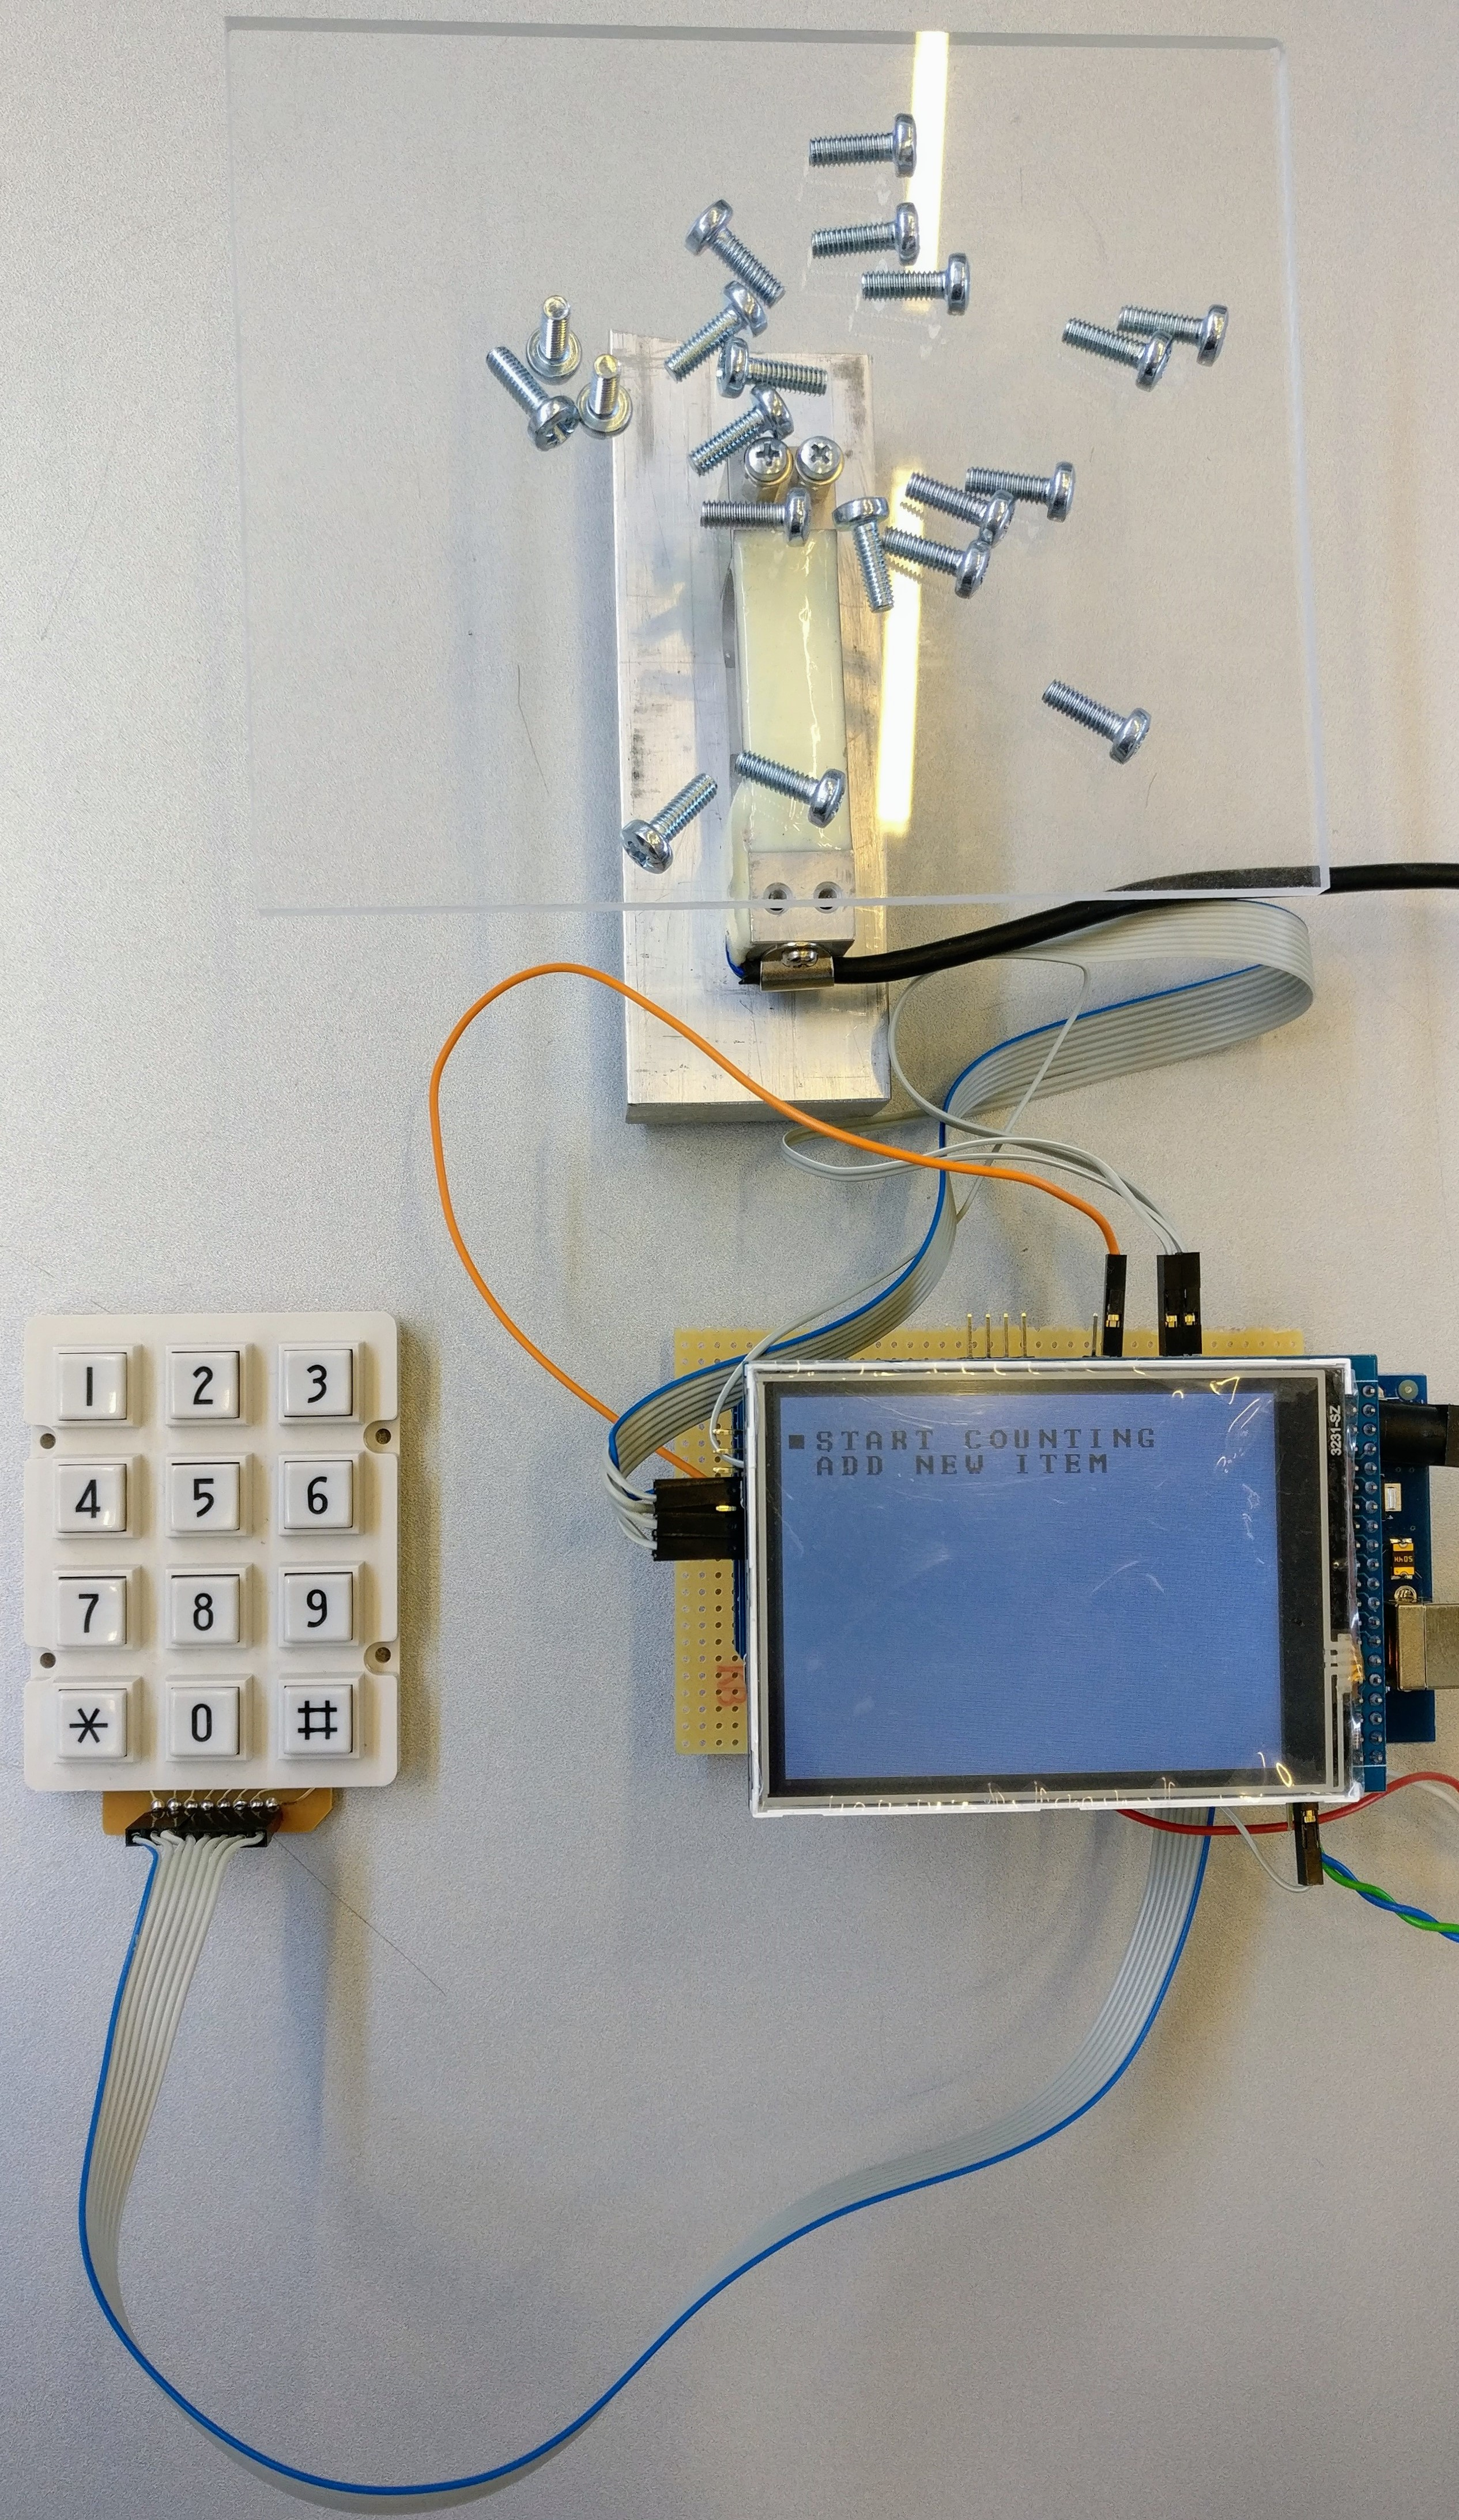
\includegraphics[width=0.4\textwidth]{graphics/frontpage}\par\vspace{1cm}
	{\Large\scshape Jonas Lind 201507296\par}
	{\Large\scshape Emil Jepsen 20092013\par}
	\vfill
	Instructor \par
	\textsc{Henning Hargaard}
	
	\vfill
	
	% Bottom of the page
	{\large \today\par}
\end{titlepage}

%-----------------------------------------------------------------
%   CONTENTS
%-----------------------------------------------------------------	
\setcounter{chapter}{1}
	
%\chapter*{Abstract}

\tableofcontents

\chapter*{Introduction}
\addcontentsline{toc}{chapter}{Introduction}
This project has been developed in the ITAMS-01 Applied Microcontroller Systems course
under instruction of Henning Hargaard. In the zipped folder \textbf{appendix}, a video demonstrating the Counting Scale system and sourcecode for the project can be found. 

\section{System Description}
This project aims to make a system that will give the user the possibility to count a number of items by weighing items on a scale. 
The user will provide a known number of items, place the items on the scale and the Counting Scale system will calculate a scaling factor. 
There are a few default items already stored in the system with a scaling factor.
With this scaling factor, the user can place an unknown number of items on the scale, and the Counting Scale system will display the number of items placed on the scale. 
In \cref{fig:system} the structure of the Counting Scale system can be seen. \\

\noindent The Counting Scale system consists of the following parts:
\begin{itemize}
	\item Arduino ATMega2560
	\item ITDB02 TFT 240RGBx320 LCD
	\item ITDB02 LCD Shield
	\item Keypad
	\item Load cell
	\item Instrumentation Amplifier
\end{itemize}

\begin{figure}[H]
	\centering
	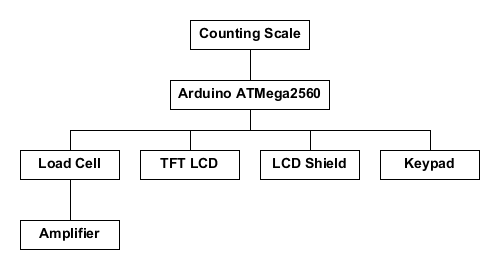
\includegraphics[width=0.6\linewidth]{graphics/system}
	\caption{Overall structure of the Counting Scale system.}
	\label{fig:system}
\end{figure}
\newpage

\noindent In \cref{fig:domainmodel} the associations between the conceptual classes of the Counting Scale system can be seen. 
The User presses a key on Keypad, the user interface, to start counting an item. 
The Arduino ATMega2560 scans the Keypad to detect if a key is pressed. 
The differential voltage from the Load Cell is gained by the Amplifier which gives a single ended output.
This signal is converted by the ADC of the Arduino ATMega2560.
The ADC output is converted to a weight and is scaled with a stored scaling factor for a given item to result in an amount of items placed on the scale.
The amount of items is displayed on the LCD.
\begin{figure}[H]
	\centering
	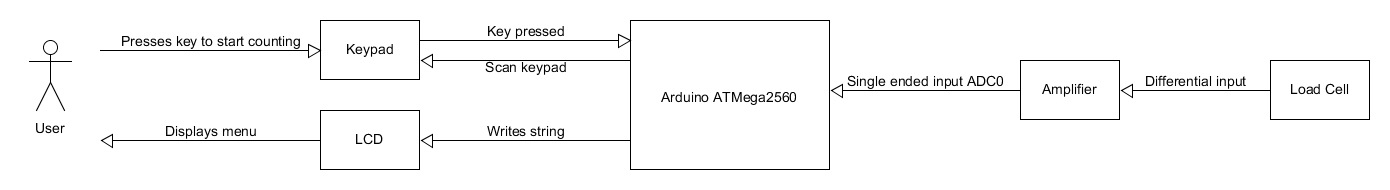
\includegraphics[width=\linewidth]{graphics/domainmodel}
	\caption{Domain Model of Counting Scale system functionality.}
	\label{fig:domainmodel}
\end{figure}

{\let\clearpage\relax \chapter*{System Architecture}}
%\chapter*{System Architecture}
\addcontentsline{toc}{chapter}{System Architecture}
The weight counter system is made with 5 different source files responsible for different parts. 
These can be seen in \cref{fig:architecture}. 
The parts are \mintinline{c}{Menu}, \mintinline{c}{TFT Driver}, \mintinline{c}{Keypad}, \mintinline{c}{Weight Counter} and \mintinline{c}{ADC}.
The menu system is called from the \mintinline{c}{main} and is responsible for the different actions of the system. 
The \mintinline{c}{Menu} system calls the state function depending on which state the menu is in. 
Then it calls the \mintinline{c}{menuStatefunc} depending on the input from the \mintinline{c}{Keypad}. The functions \mintinline{c}{getLetter} and \mintinline{c}{getNumber} is used when the user needs to enter a letter and number respectively. 
The menu system uses the \mintinline{c}{TFT Driver} to output information to the display using the \mintinline{c}{write} and \mintinline{c}{ClearArea} functions. 
The menu system uses the keypad function \mintinline{c}{NumKeyScan} to get the input from user.  
The menu uses \mintinline{c}{Weight Counter} function \mintinline{c}{Counter} when the weight cell is used as a weight counter. 
The \mintinline{c}{ADC_single_avg} is called from \mintinline{c}{Menu} when the user wants to add a new item to the weight counter. 
The function then measures the weight of the item.

\begin{figure}
\centering
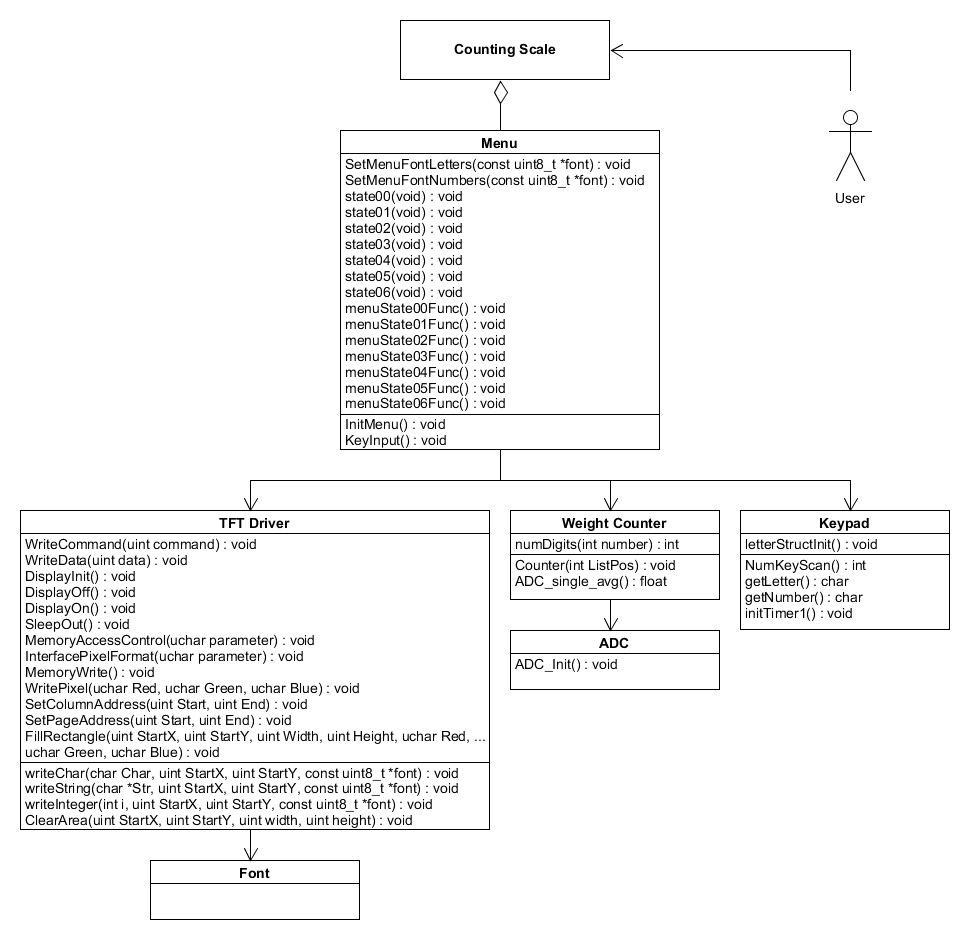
\includegraphics[width=1\linewidth]{graphics/architecture}
\caption{Software architecture of the Counting Scale system. Functions below the line are used in other source files while functions above the line are only used in their own respective sourcefile.}
\label{fig:architecture}
\end{figure}


\chapter*{System Design}
\addcontentsline{toc}{chapter}{System Design}
\section{Load Cell}
The load cell used in this project is a MP40/10 N. \cite{DS-MP40} 
It has a max. capacity of \SI{1}{\kilogram} making it suitable for a counting scale used to count small pieces, e.g. screws. 
The load cell has a rated output of \SI{1}{\milli\volt/\volt}.
The maximum supply voltage for the load cell is \SI{15}{\volt}, but it was chosen to use a \SI{5}{\volt} supply from the Arduino ATMega2560 board. 
This was done as a project delimitation to avoid using more than one voltage supply for the system. \\

The voltage output from the load cell depends on the supply voltage. 
This will require a constant voltage supply. 
To compensate for voltage dips, short interruptions or ripple in the supply voltage, a reference voltage is given to the analog reference pin, \mintinline{c}{AREF} for the ADC. 
The output is hereby ratiometric to the supply voltage.

\begin{figure}[H]
	\centering
	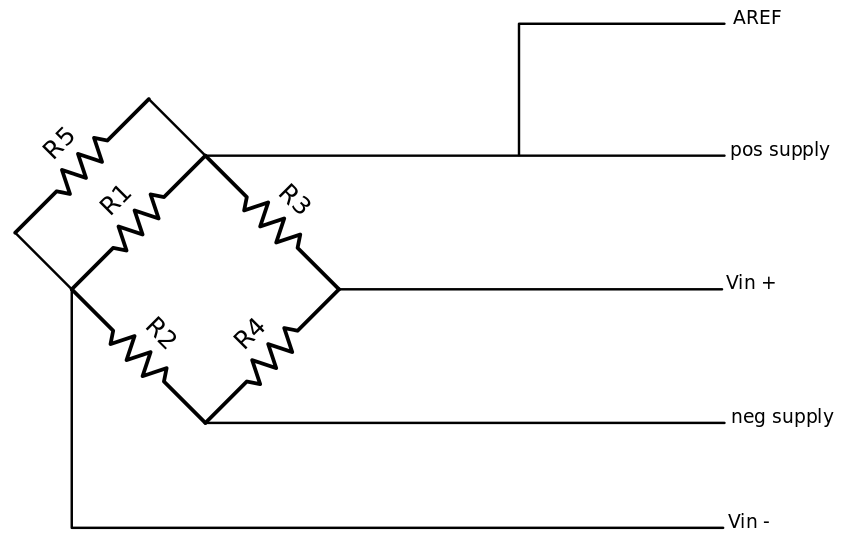
\includegraphics[width=0.6\linewidth]{graphics/loadcell}
	\caption{Ratiometric measurement.}
	\label{fig:loadcell}
\end{figure}

The load cell had an offset of $\approx\SI{28}{\milli\volt}$ at first. 
This was corrected by trimming resistor R1 in the wheatstone bridge using a parallel resistor R5 as seen on \Cref{fig:loadcell}.
When resistor R5$=\SI{51}{\kilo\hertz}$, the offset became $\approx \SI{600}{\micro\volt}$. 

\subsection{Amplifier}
With a voltage supply of \SI{5}{\volt} the output will be \SI{5}{\milli\volt}.
To use the full dynamic range of the ADC, an amplifier is needed to amplify the output.
The Arduino Atmega2560 has built-in channels for differential input with different sets of gain between $10\times$ and $200\times$.
When using $200\times$ gain, only 7 bit resolution can be expected. \cite[p.~268]{ATmega2560}
This gives a poor resolution and the gain is not sufficient to use the entire dynamic range of the ADC. 
If the gain had been selected as $200\times$, a voltage divider could have been used to lower the voltage at the \mintinline{c}{AREF} pin.
Instead of using the differential input channels with built-in gain, the instrumentation amplifier INA125P with precision voltage reference is used in this project. \cite{INA125}

\begin{equation}
G = 4+\frac{\SI{60}{\kilo\ohm}}{R_G}=\frac{\SI{60}{\kilo\ohm}}{\SI{82}{\ohm}} \approx 735
\label{eq:gain}
\end{equation}

The gain of the amplifier must be set to a value securing that the full dynamic range of the ADC is used. 
The gain of the amplifier is set to $735\times$, see \cref{eq:gain}. 
With this gain the offset becomes $\approx \SI{450}{\milli\volt}$ and will result in the ADC input range being $\approx \text{\SI{450}{\milli\volt}}+\SI{3.7}{\volt}\approx\SI{4.15}{\volt}$.
With this gain not the entire dynamic range of the ADC is used, but leaves some heading for eventually drifting. 
The gain could perhaps have been placed higher, as long the ADC input range would not exceed \SI{5}{\volt}, see \cref{eq:inputrange}.

\begin{equation}
(\text{Rated Output}+\text{Offset})\cdot G < \SI{5}{\volt}
\label{eq:inputrange}
\end{equation} 

\subsection{ADC Configuration}
The ADC converts the input voltage to a 10-bit value.
The minimum ADC value represents GND and the maximum ADC value represents the voltage on the AREF pin, minus 1 LSB.\cite[p.~269]{ATmega2560}
A single ended channel is used with the output of the instrumentation amplifier connected to \mintinline{c}{ADC0} on the Arduino ATMega2560 board. 

\paragraph{\mintinline{c}{ADMUX}} 
To select \mintinline{c}{ADC0} as input channel the \mintinline{c}{MUX} bits are set low in the \mintinline{c}{ADMUX} register.
To select \mintinline{c}{AREF} to external voltage reference, the \mintinline{c}{REFS} bits are set low.

\paragraph{\mintinline{c}{ADCSRA}}
To select the input clock to the ADC the \mintinline{c}{ADPS} bits are set high in the  \mintinline{c}{ADCSRA} register. 
These bits specify the division factor used to divide the CPU frequency. 
With a CPU frequency of \SI{16}{\mega\hertz}, a division factor of 128 will result in a input clock to the ADC of \SI{125}{\kilo\hertz}, see \cref{eq:adcclock}.
Enabling the ADC is done by writing the \mintinline{c}{ADEN} bit.

\begin{equation}
\text{ADC Clock}=\frac{\SI{16}{\mega\hertz}}{128}=\SI{125}{\kilo\hertz}
\label{eq:adcclock}
\end{equation}

\paragraph{\mintinline{c}{ADCSRB}}
To select \mintinline{c}{ADC0} as input channel the \mintinline{c}{MUX5} bit are set low in the \mintinline{c}{ADCSRB} register.\\

\noindent See datasheet for ADC register decriptions. \cite[p.~281-288]{ATmega2560}

\begin{lstlisting}[caption={Initialization of ADC.}, label={lst:ADC},language=C++,directivestyle={\color{black}},
emph={int,char,double,float,unsigned},emphstyle={\color{blue}}]
void ADC_Init()
{
	// AREF; Single Ended Input ADC0
    ADMUX = 0b00000000;
    // ADC Enable; ADC Prescaler = 128
    ADCSRA = 0b10000111;
    ADCSRB = 0b00000000;
}
\end{lstlisting}


\subsection{Count Scale Configuration}
The count scale is configured after measuring a trendline made by placing different weights upon the load cell and then reading the ADC value. 
The offset can be seen as 92 ADC counts and correspond well with the offset of \SI{450}{\milli\volt} when the ADC has a resolution of \SI{4.88}{\milli\volt}, \cref{eq:resolutionvoltage}. 
The resolution can also be specified in grams as seen in \cref{eq:resolutiongrams}.

\begin{equation}
\text{Resolution}=\frac{\SI{5}{\volt}}{2^{10}}= \SI{4.88}{\milli\volt}
\label{eq:resolutionvoltage}
\end{equation}

\begin{equation}
\text{Resolution}=\frac{\text{Weight}}{\text{ADC Count}-\text{ADC Offset}}=\frac{\SI{500}{\gram}}{462-92}=\SI{1.35}{\gram}
\label{eq:resolutiongrams}
\end{equation}

\begin{figure}[H]
	\centering
	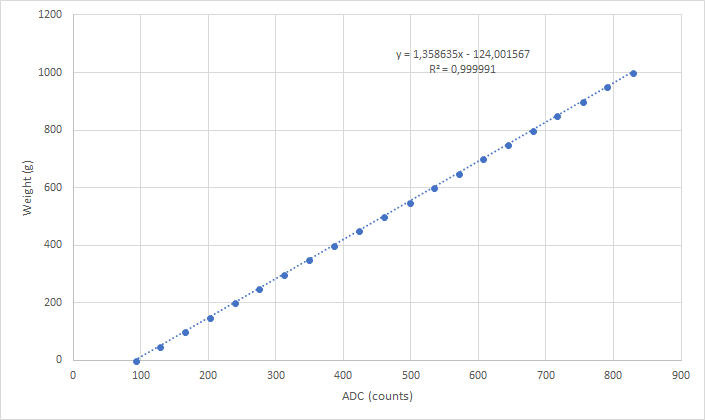
\includegraphics[width=0.67\linewidth]{graphics/loadcellconfig}
	\caption{Configuration of load cell.}
	\label{fig:loadcellconfig}
\end{figure}
\vspace{-25pt}
\begin{equation}
y = 1.3586-124
\label{eq:trendline}
\end{equation}

With this trendline, \cref{eq:trendline}, the weight corresponding to a given ADC count can be calculated.
The weight is averaged over 5 measurements to give a more steady output to avoid number flickering on the graphic display.
The amount is calculated by dividing the weight with a scaling factor given by the items weight divided by the amount of items specified by the user. 
\vspace{-15pt}
\begin{lstlisting}[caption={Amount of items calculated with use of the trendline.}, label={lst:counter},language=C++,directivestyle={\color{black}},
emph={int,char,double,float,unsigned},emphstyle={\color{blue}}]
void Counter(int ListPos)
{
	volatile int amount;
	volatile float weight;
	...
	ADC_avg += ADCW;
	count ++;
	if (count == 5)
	{
	    ADC_avg = ADC_avg / 5;
	    weight = (ADC_avg * 1.3586) - 138; // Change in offset
	    amount = (int) (weight / WeightList[ListPos]);
	    ADC_avg = 0;
	    count = 0;
	    _delay_ms(20);
	}
}
\end{lstlisting}
\section{Keypad}
To take user input a keypad with 12 keys is used, see \cref{fig:keypad}. \cite{rspro} 
This was chosen to have a simple user interface for the user to input numbers and has been extended to handle input as letters also.
There is a long delay after the button has been released until the output is changed. 
This means there is added a delay in different parts of the code to make sure enough time has passed for the keypad to change. 
Another possibility would be using the touch screen of the graphic display. 
It could have been implemented with a variable amount of keys shown on the display. 
This would reduce the number of components since the touchscreen is already a part of the display. 
The downside of using the screen for user input is that it takes up space on the display. This means there is less space for showing relevant information for the user.

\begin{figure}[H]
\centering
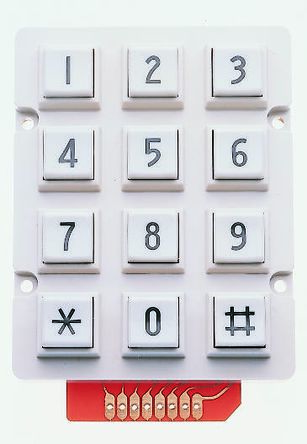
\includegraphics[width=0.3\linewidth]{graphics/keypad}
\caption{The keypad is the user interface to get input from the user. Square button is used as enter and star button is used to delete input.}
\label{fig:keypad}
\end{figure}


\subsection{Keypad Scan}
The keypad has its keys placed in a $4\times3$ matrix layout. 
There are 8 pins with 4 rows, 3 columns and 1 SC pin connected to ground. 
The 3 column pins are set high one at a time by bit shifting through \mintinline{c}{PORTL} bit \mintinline{c}{2, 1, 0}. 
The 4 row pins are pulled to ground with pull down resistors.
When a key is pressed a connection between a column, which is high, and a row which is low will happen.
This will set the row high. 
The 4 row pins are set as inputs, with one row checked at a time by bit shifting through \mintinline{c}{PINL} bit \mintinline{c}{7, 6, 5, 4}. \cite{matrixkeypad}
The \mintinline{c}{NumKeyScan} function returns a number between 1-12, with 1 = 1, 2 = 2, ..., \# = 12. 

\subsection{Keypad Numbers}
To use the keypad for numbers only, the input from the keypad scan is added with 48 turning the input to the corresponding ASCII numbers. The numbers are shown on the display with a large font as each number is entered. The number is then stored in a char array which is used when the user has finished entering numbers. To delete numbers the star key has been chosen. This deletes the number from the display and from the char array.

\subsection{Keypad Letters}
To use the keypad to enter letters or numbers, it is used as an telephone keypad according to the international standard. \cite{keypad} This means the number 2 also represents a, b and c. Every key has a struct containing the different possible characters. It also contains the amount of characters and the current position. 
A timer is implemented using an interrupt. If there has been a keypad input with the same value as before and the timer is lower than the threshold, the position is moved. The corresponding letter is then shown on the display. If a new key is pressed the timer is reset. The threshold is set at \SI{2}{\second} to make sure the user has time to input a new character. The keypad is quite slow mechanically so a longer delay is required. The characters selected by the user is shown on the display as text when the user presses a key. If it is pressed before the timer runs out the old character is overwritten with a new character. The star key has been chosen to delete characters if pressed. The name is stored in a char array until the user is finished inputting the letters.

\section{Graphic Display}
It has been chosen to use a graphic display to show the user interface. 
The advantage of this is the much larger screen, this gives more choices in making the menu system. 
Another advantage is the possibility  to show larger numbers on the screen making the weight counter easier to use. 
This is a big difference compared to a $2\times20$ LCD which is much more limited in what can be displayed on the screen.

The graphic display used in this project is a ITBD02 display. \cite{TJC}
This is implemented with a ILI9431 controller. \cite{ILI9413} 
It is a $320\times240$ pixel display. In this project it is using a 16 bit interface. 
The coloring is done using RGB where bits \mintinline{c}{0-4} is for blue, bit \mintinline{c}{5-10} is for green and \mintinline{c}{11-15} is for red. 
This means the RGB is transferred as \mintinline{c}{5-6-5} for blue, green and red.
When writing commands to the driver it is done by transferring 8 bits. 
There is a 16 bit parallel bus for transferring data or commands. 
Since the display uses \SI{3.3}{\volt}, an TDB02 Arduino MEGA shield is used as in intermediate between the ATMega2560 and the display.

The driver is implemented with the \mintinline{c}{writecommand} and \mintinline{c}{writeData} functions implemented according to \cite[p.~238]{ILI9413}. 
To send data or commands the \mintinline{c}{chipselect(CSX)} is set low. 
The \mintinline{c}{DCX} is set low to write a command and it is set high to write data. 
The \mintinline{c}{WRX} pin is a write pin. 
On rising edge it writes data or command. 
This means \mintinline{c}{WRX} is first set low then held low for at least \SI{15}{\nano\second} and is then set high and held high for at least \SI{10}{\nano\second}. \cite[p.~10 \& 238]{ILI9413}
One \mintinline{c}{NOP} instruction gives a delay of \SI{62.5}{\nano\second} since the the clock frequency is \SI{16}{\mega\hertz}. 
The display is initialized by resetting it using the \mintinline{c}{RESX} pin by setting it low, holding it low and then setting it high.
Then there must be a delay of at least \SI{120}{\milli\second} until the display has finished the blanking sequence. \cite[p.~230]{ILI9413}
Then the sleep mode is exited and the display is set to on.
The display is set to use RGB colors and switch column and rows. 
The pixel format is set to 16 bit.

An interesting function is the \mintinline{c}{writeChar}. It is based on a TFT driver for Arduino by Henning Karlsen\cite{UTFTLIB}.
The function \mintinline{c}{writeChar} takes a character and the start positions x and y as inputs. 
The last input is a pointer to a font. 
This font describes the style and size of the character shown on the display. 
The font must be stored in flash memory of the ATMega2560. 
Since the ATMega2560 has much more limited amount of RAM than flash memory, the constant font lies in flash memory which also is where the program is stored. \cite[p.~20]{ATmega2560}
To store constant data in program memory the \mintinline{c}{PROGMEM} identifier is used. \cite{progmem} 
This will store the data in program space. It is not possible to access constant data in program memory directly since the pointer returns the address in RAM memory and not in program memory. 
The macro available to read data in program space is \mintinline{c}{pgm_read_byte} used for a byte. 
This reduces speed very little, but has the advantage that a much larger number of fonts can be used.
Otherwise the fonts would be smaller and have fewer characters. 

The fonts need to have a specific format. 
The format used has as the first entry a width, the second a height, the third a offset of the font's first character compared to the ASCII values and the fourth the number of characters the font has. 
Every entry in the fonts is a char which describes whether a pixel is on or off. 
The chars are combined to make a line depending on the width of the char. 
See \cref{lst:writechar} for \mintinline{c}{writeChar} where the size and ASCII offset is read. 
The end addresses is set from the size of the font. 
The \mintinline{c}{Charpos} is the entry in the font array and is calculated using the size and the fact that char has a size of 8 bits. 
All bits are then read and checked if it is 1. 
If the bit is set, a black pixel is written on the screen otherwise a white pixel is written on the screen. The fonts are downloaded from \cite{UTFT}.
\vspace{-20pt}
\begin{lstlisting}[caption={\mintinline{c}{writeChar} function.}, label={lst:writechar}, language=C, directivestyle={\color{black}},
emph={int,char,double,float,unsigned}, emphstyle={\color{blue}}]
void writeChar(char Char, unsigned int StartX, unsigned int StartY,
const uint8_t *font)
{
	uint8_t y_size = pgm_read_byte(&font[0]);
	uint8_t x_size = pgm_read_byte(&font[1]);
	uint8_t ascii_offset = pgm_read_byte(&font[2]);
	SetPageAddress(StartX, StartX + x_size - 1);
	SetColumnAddress(StartY, StartY + y_size - 1);	
	MemoryWrite();
	uint16_t Charpos = (Char -  ascii_offset) * ((y_size/8)*x_size) + 4;
	uint16_t temp = (y_size/8)*x_size;
	uint8_t bits_to_show;
	for(int i=0; i < temp; i++)
	{
		bits_to_show = pgm_read_byte(&font[i+Charpos]);
		for(uint8_t j=0; j<8;j++)
		{
			if(bits_to_show >> (7-j) & 1)
			{
				WritePixel(0, 0, 0);
			}
			else
			{
				WritePixel(31,63,31);
			}
		}
	}
}
\end{lstlisting}
It has been decided to use a white screen as background which means that every time text needs to be cleared it is just overwritten with white. For the font type used for text see \cref{fig:StartMenuScreen} and for font used for numbers see \cref{fig:NoItems}.
The font for numbers is much larger since the amount of numbers shown is smaller. This also have the advantage that the amount is much easier to see when using the weight counter.




\section{Menu}
The user interface is based on a menu system where the user can navigate using a keypad. The menu system is implemented as a state machine. This is done by using two different switch statements. The first is \mintinline{c}{KeyInput} which calls the function corresponding to the current \mintinline{c}{menuState} the menu is in. The state function are updating the \mintinline{c}{menuState} depending on the input from the user. 
It is changed to the state corresponding to the selected part of the menu.

\begin{lstlisting}[caption={The statemachine of menu system.}, label={lst:menu}, language=C,directivestyle={\color{black}},
emph={int,char,double,float,unsigned},emphstyle={\color{blue}}]
void KeyInput(void)
{
	switch(menuState)
	{
		case 0:
			state00();
			break;
		case 1:
			state01();
			break;
		case 2:
			state02();
			break;
		case 3:
			state03();
			break;
		case 4:
			state04();
			break;
		case 5:
			state05();
			break;
		case 6:
			state06();
			break;
	}
	// reset global variable so that we know the input is dealt with
	_delay_ms(10);
	keyPushInput = KEY_NULL;
}
\end{lstlisting}
\vspace{10pt}
The \mintinline{c}{menuState} functions are responsibly for the action of that \mintinline{c}{menuState}. This could be showing new information on the screen or running the ADC and outputting the result.
\newpage
\begin{lstlisting}[caption={Implementation of the states in the menu system.}, label={lst:menustate}, language=C,directivestyle={\color{black}},
emph={int,char,double,float,unsigned},emphstyle={\color{blue}}]
// Start count
void state00(void)
{
	switch(keyPushInput)
	{
		case KEY_UP: // Change to state04
			menuState = 3;
			LCDChange = 1;
			menuState03Func();
			break;
		case KEY_DOWN: // Change to state02
			menuState = 3;
			LCDChange = 1;
			menuState03Func();
			break;
		case KEY_STAR: // Do nothing
			break;
		case KEY_SQUARE: // Call menuState01
			menuState = 1;
			LCDChange = 1;
			ListPosition = 0;
			menuState01Func();
			break;
		default: // Do nothing
			break;
	}
	keyPushInput = KEY_NULL;
}
\end{lstlisting}
The changing of \mintinline{c}{menuState} is done in the different state functions. Since the menu only has a few menu states it is possible to do this without it being too complicated. The downside of doing it this way, is when adding new menu states. Adding new menu states requires changing the state functions so the menu state is connected directly to each other. This is done in different functions which makes it more complicated.

The menu system will show multiple options which the user can choose between. The different options will be shown on the screen at the same time. The starting display is showing the following as seen on \cref{fig:StartMenuScreen}.

\begin{figure}[H]
	\centering
	\subfloat[Start menu is showing the two options, start counting which leads to a list of items for using the weight as a weight counter.]{
\includegraphics[width=.48\textwidth]{graphics/StartMenuScreen}\label{fig:StartMenuScreen}}
	\hfill
	\subfloat[The list of items to choose between when using the weight counter.]{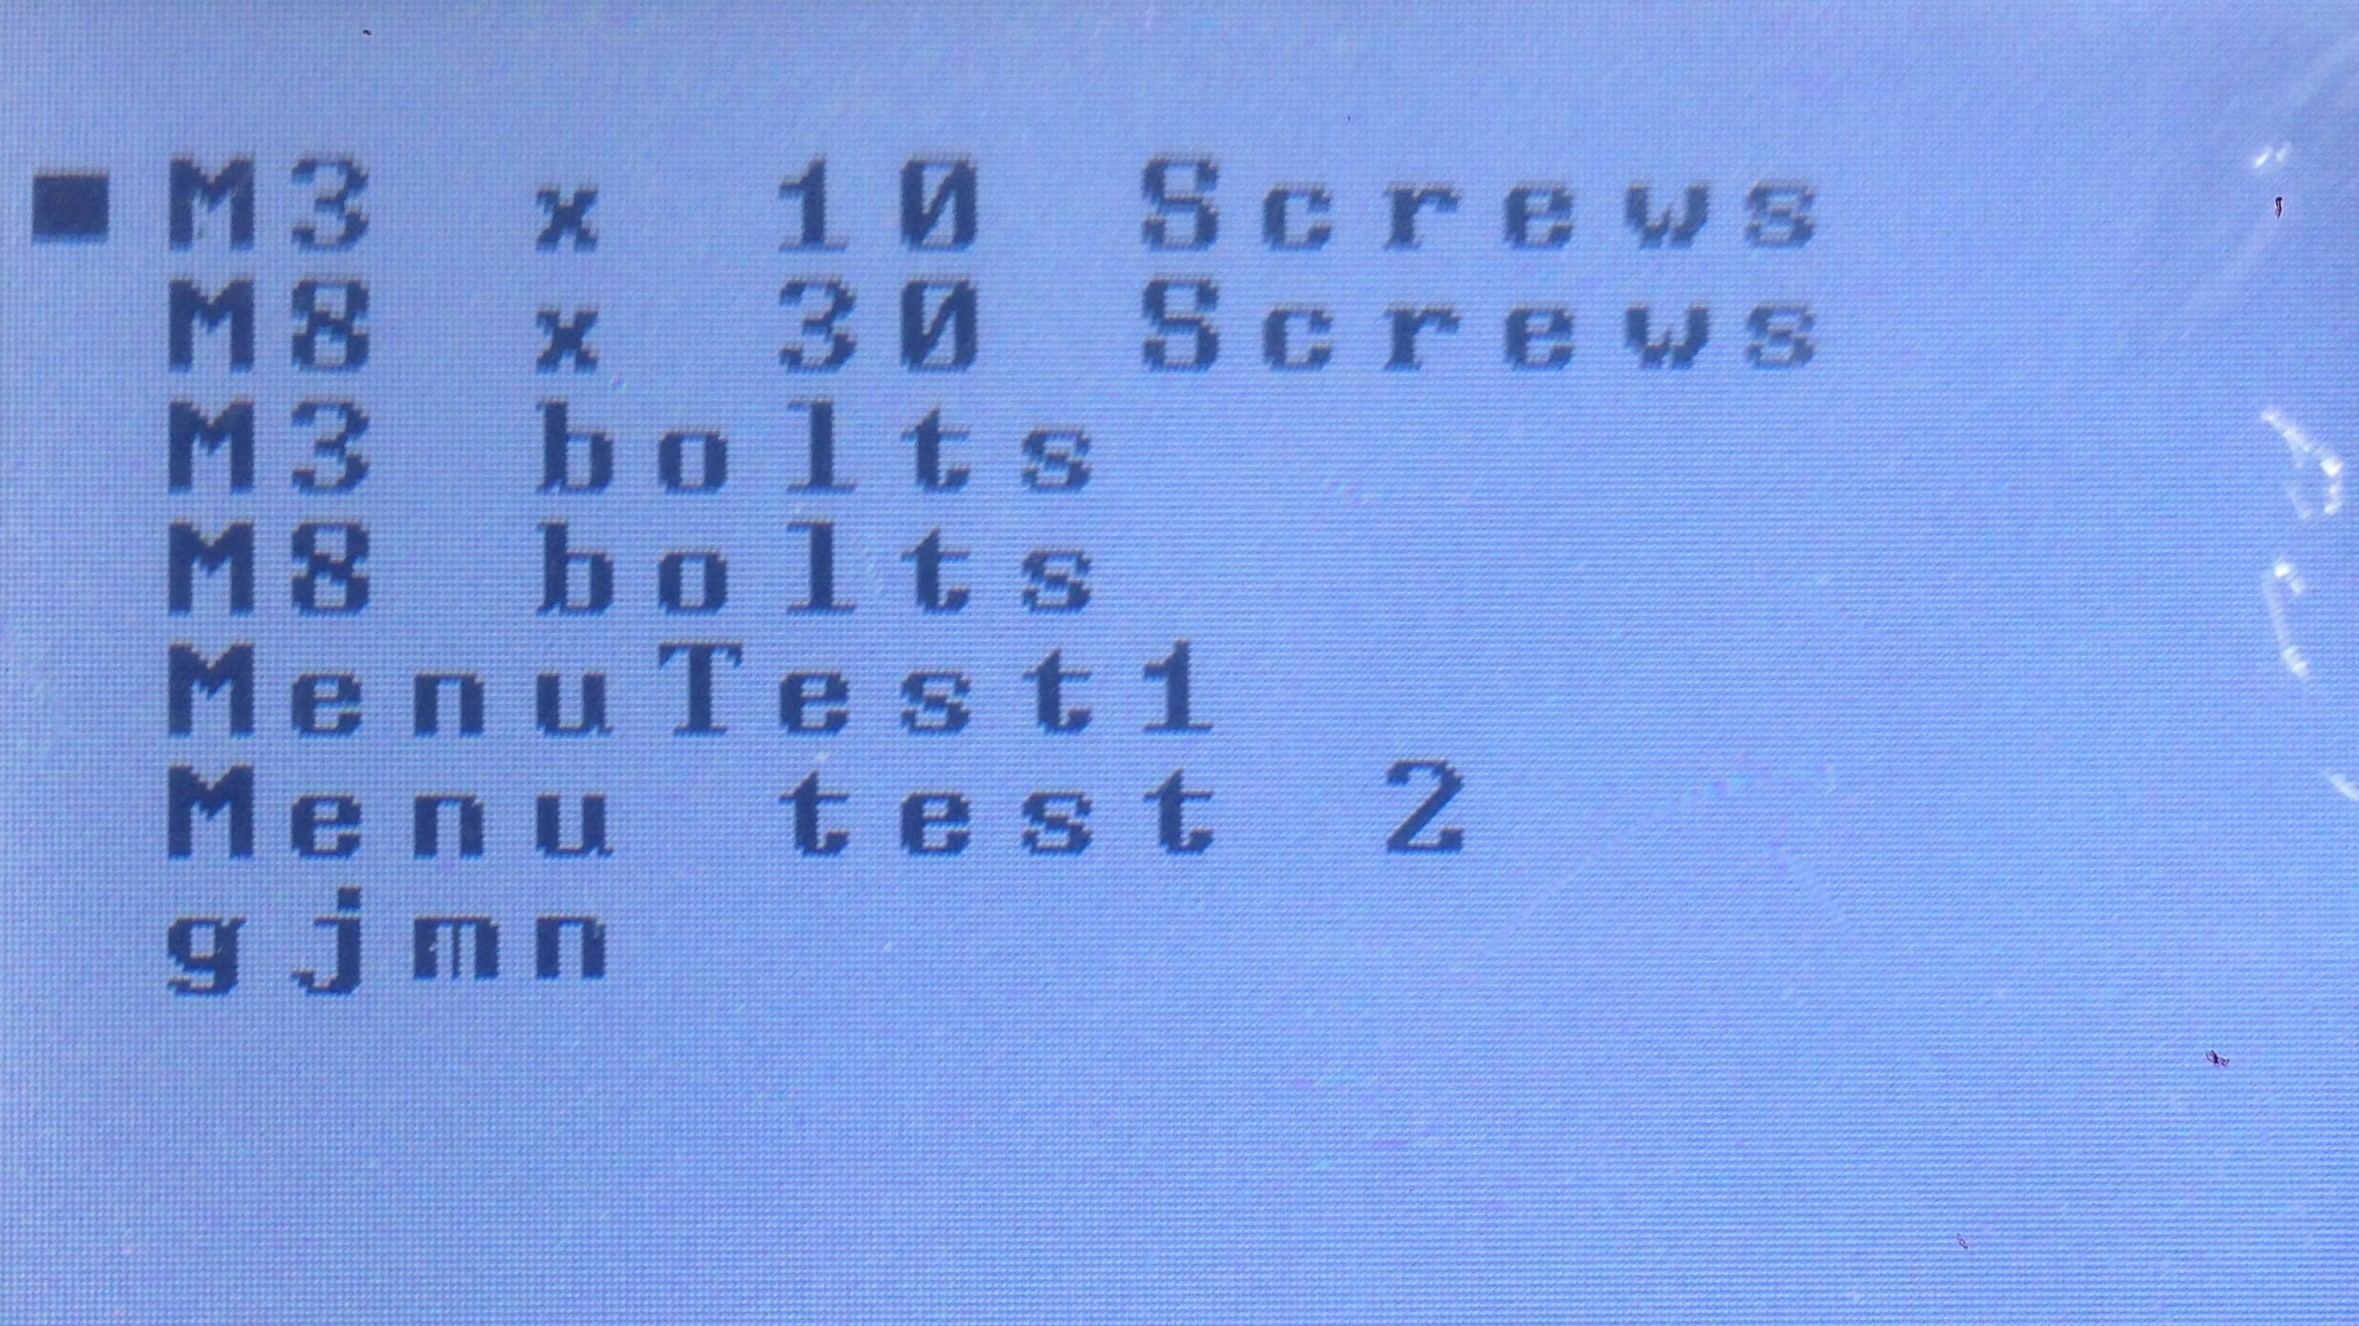
\includegraphics[width=.48\textwidth]{graphics/ListObjects}\label{fig:ListObjects}}
	\caption{Menu showing start menu and list of items menu.}	
\end{figure}


The black dot indicates the menu item which will be selected if the user presses the square key. If the user chooses start counting the output on the display can be seen in \cref{fig:ListObjects}. The display  will show as many menu items as there can fit in one column on the screen. If the chosen item will move outside the list then the whole list moves in the corresponding direction instead.

\begin{figure}[H]
	\centering
	\subfloat[Screen showing when the weight counter is selected and the item is selected.]{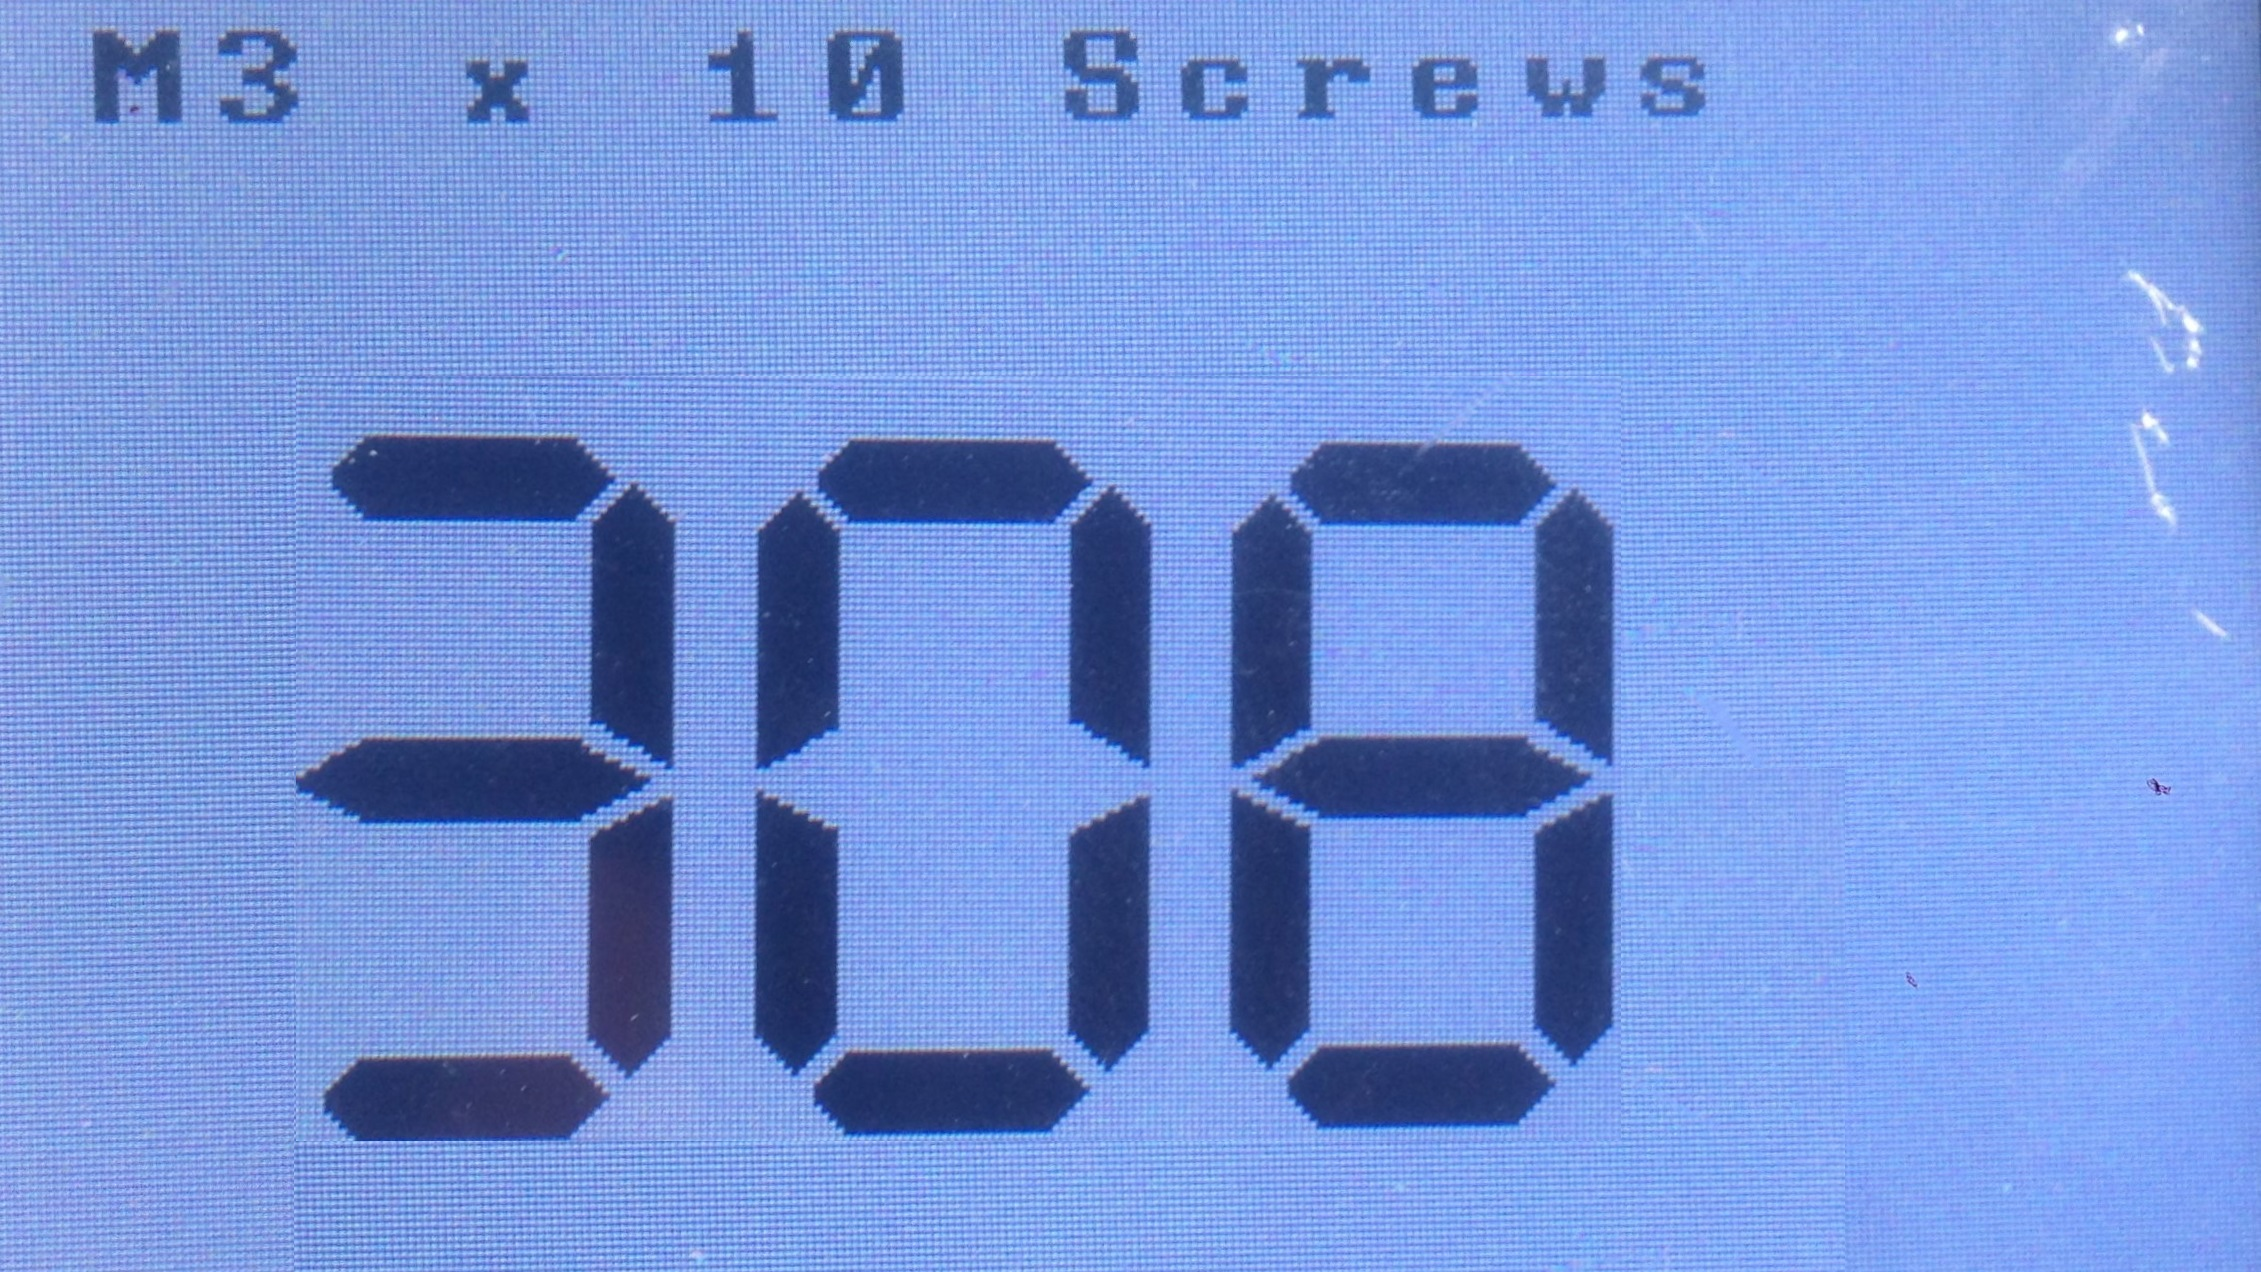
\includegraphics[width=.48\textwidth]{graphics/WeightCount}\label{fig:WeightCount}}
	\hfill
	\subfloat[The User can enter the name of a new item to be added. This item can be used with the weight counter.]{
\includegraphics[width=.48\textwidth]{graphics/EnterName}\label{fig:EnterName}}
	\caption{Menu showing weight menu and new item name menu.}	
\end{figure}

When the item is selected by the user, the weight counter screen is shown see \cref{fig:WeightCount}. This is done by calling the \mintinline{c}{Counter} function. 
If the user selects add new item in \cref{fig:StartMenuScreen} the display will show a prompt for the user to enter the name for the new item, see \cref{fig:EnterName}.
The user can enter the name using a keypad. It is possible to delete already entered characters. When the user is finished inputting the name, the square button will proceed to the next part. The next part can be seen in \cref{fig:itemsOnScale}. The user is told to place a number of the items to be added to the weight counter.

\begin{figure}[H]
	\centering
	\subfloat[The user is told to place items on scale so an average weight of the item can be calculated.]{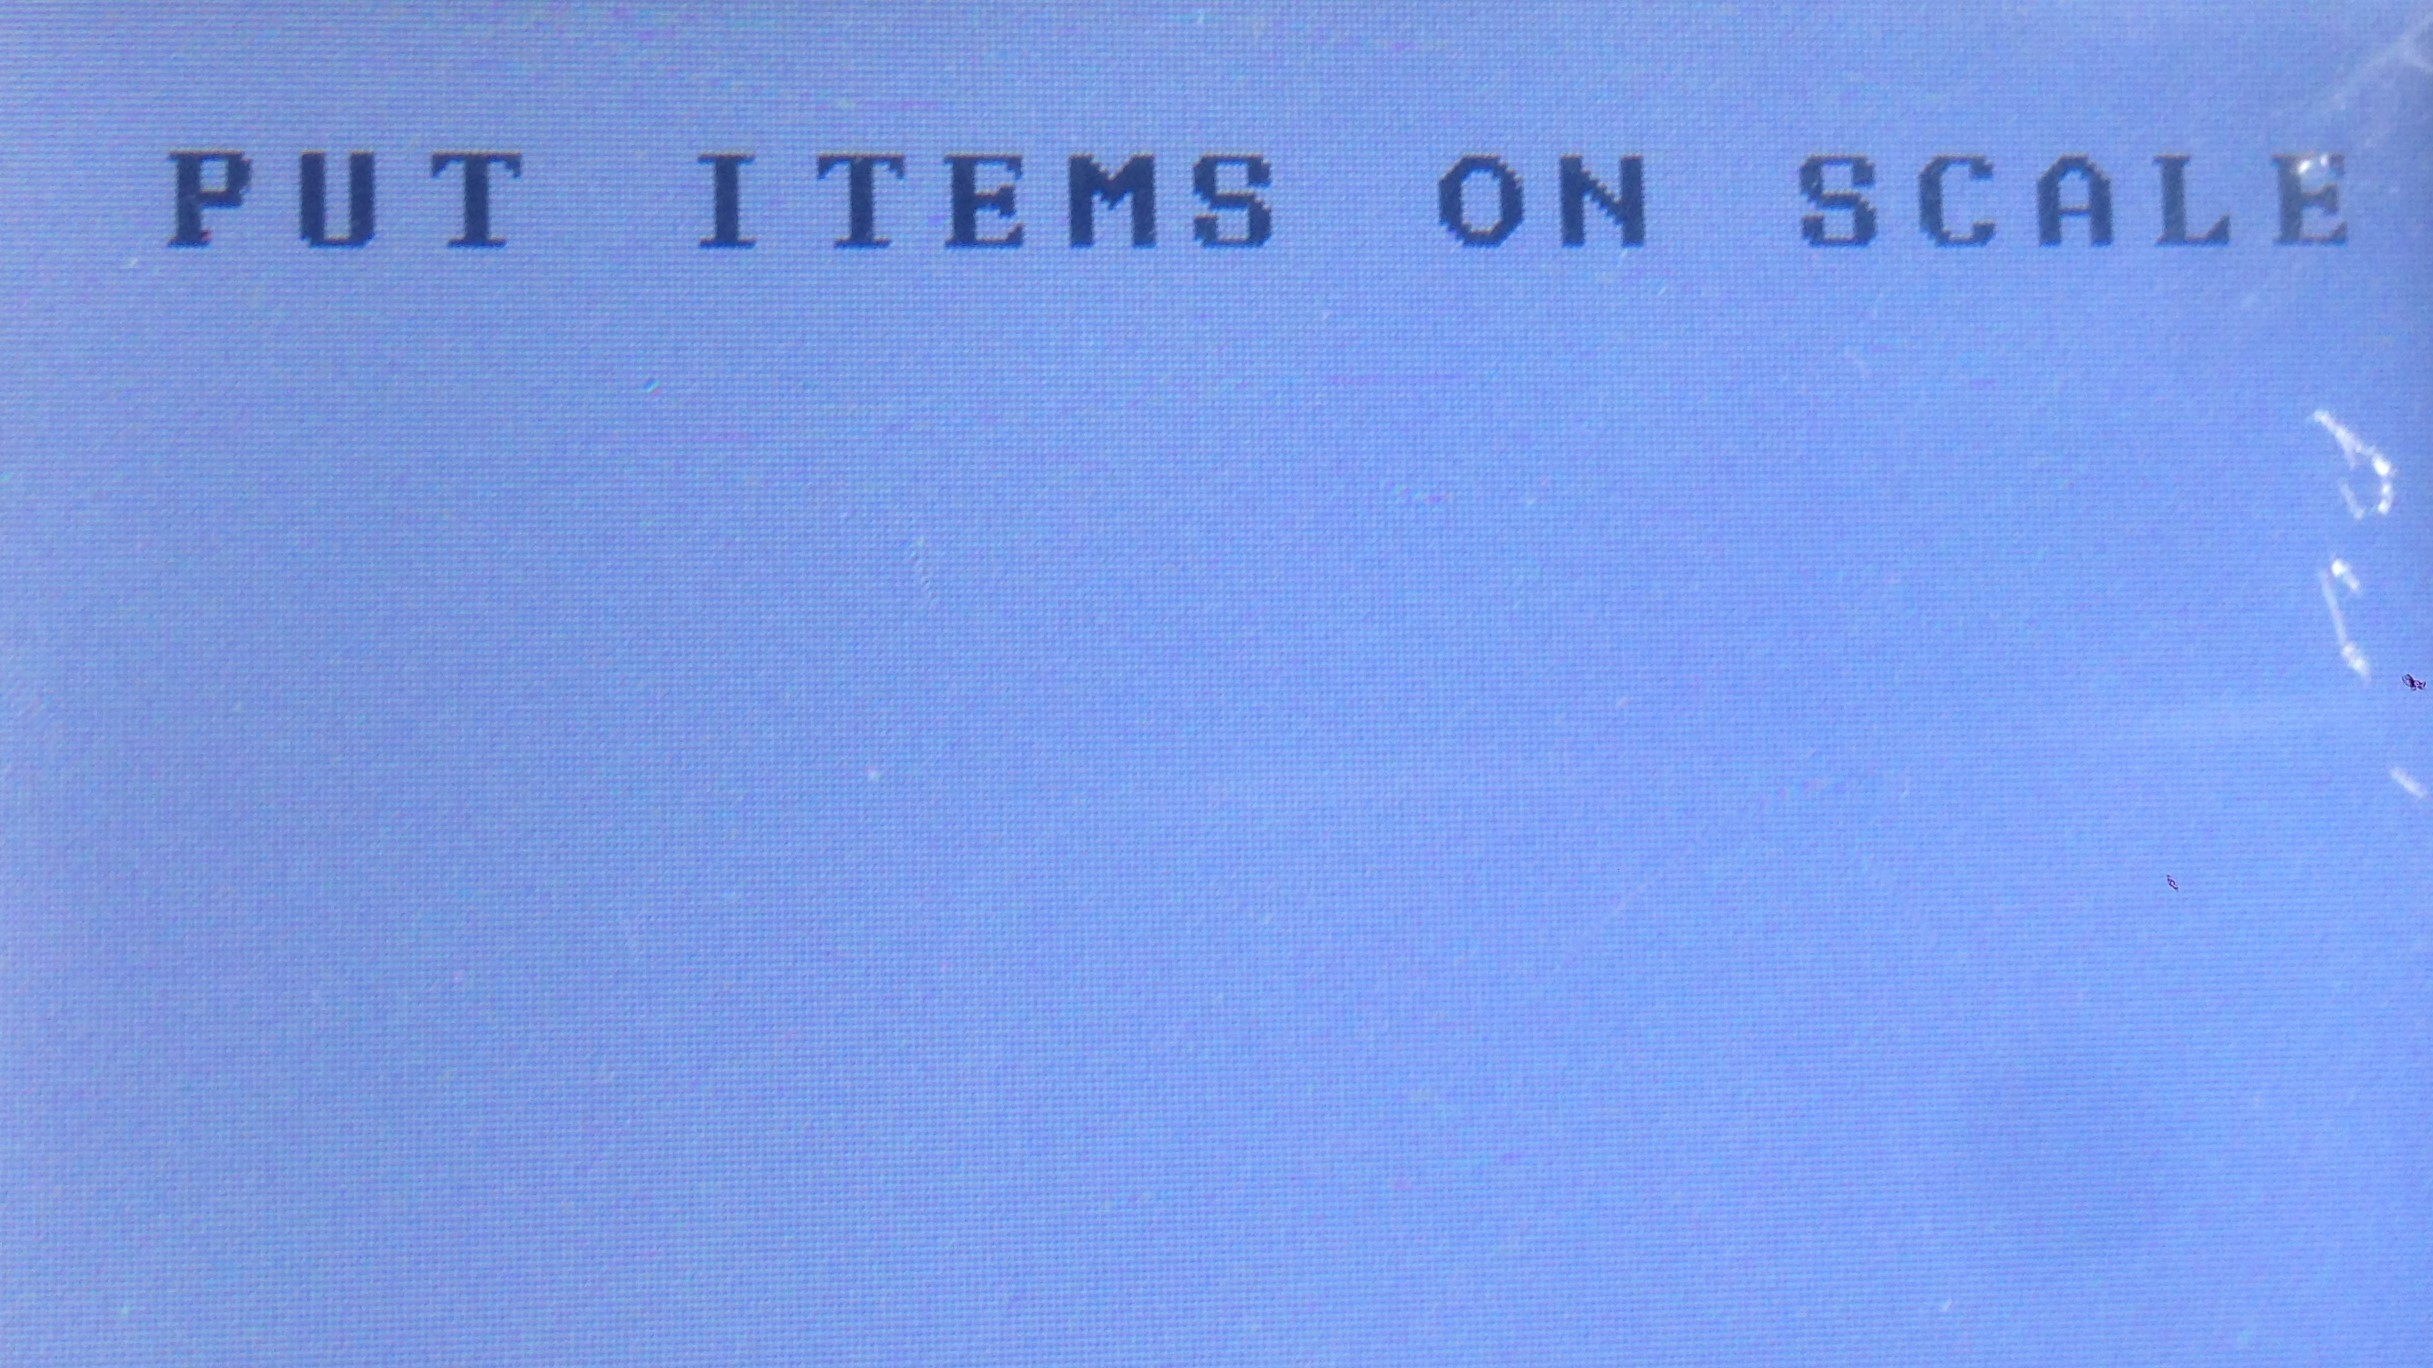
\includegraphics[width=.48\textwidth]{graphics/itemsOnScale}\label{fig:itemsOnScale}}
	\hfill
	\subfloat[The User can enter the name of a new item to be added. This item can be used with the weight counter.]{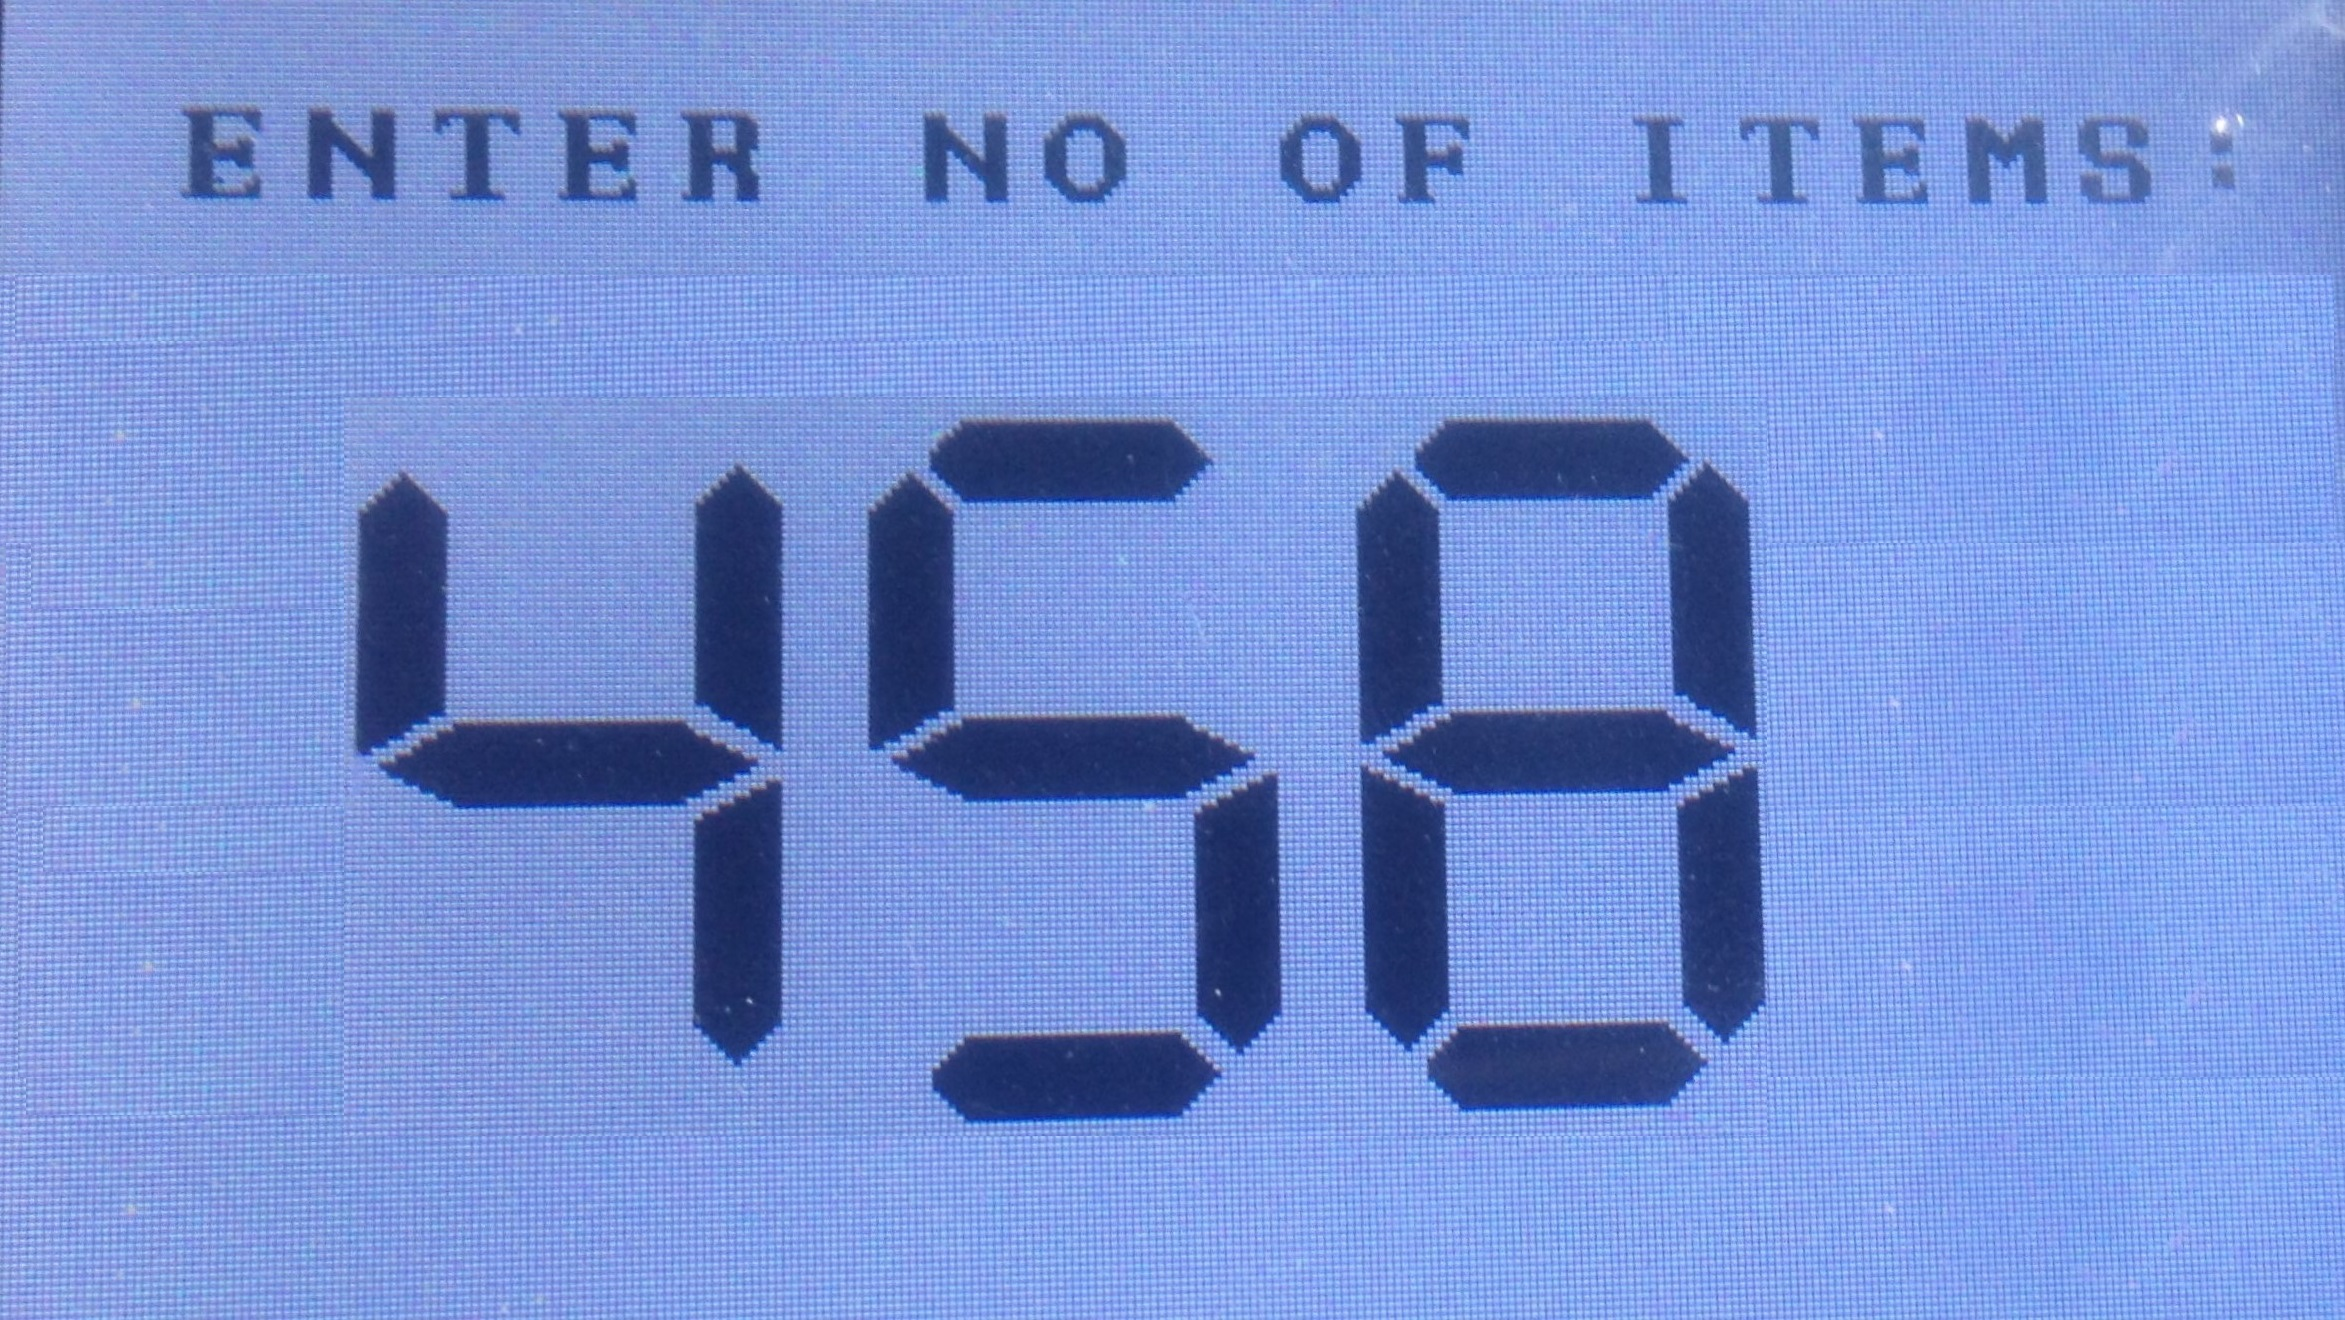
\includegraphics[width=.48\textwidth]{graphics/NoItems}\label{fig:NoItems}}
	\caption{Menu showing instruction to out items on scale menu and instruction to enter number of items menu.}	
\end{figure}

When the items are placed on the scale, the user continues to the next screen which can be seen on \cref{fig:NoItems}. The user enter how many items have been placed on the scale. When the amount has been entered, the name and average weight is stored permanently in memory even if the device is powered off.

This is done by using the eeprom feature of the ATMega2560. The eeprom is non volatile with $100\,000$ write cycles. The advantage of using eeprom compared to flash memory is that the program is placed in flash memory. Placing the data in flash would require part of it to only hold the data and not the program. The eeprom is currrently unused so it is simpler to implement. The other advantage is more write cycles for the eeprom than flash, $100\,000$ compared to $10\,000$. It is unlikely to use this many writes to non volatile memory in this application. Another advantage is the ability of eeprom to be accessed as bytes where flash can only be accessed as pages. Since the data being accessed is quite small, eeprom has the ability to only read or write the required data. The eeprom is implemented using the avr-libc library eeprom. \cite{EEPROM} The functions that are used with eeprom can be seen in \cref{lst:eeprom}. The \mintinline{c}{eeprom_update_block} saves the new name and \mintinline{c}{eeprom_update_float} saves the average value in eeprom. At the start up of the weight counter data is transferred from eeprom to RAM since it is slower to read data from eeprom than getting data from RAM. This is done by using the functions \mintinline{c}{eeprom_read_block} and \mintinline{c}{eeprom_read_float} for the name and average weight respectively. The block functions allows the transfer of a variable length of bytes. The type these functions take is void pointers which means the type of data is not used by the function allowing all types to be transferred.
\vspace{-10pt}
\begin{lstlisting}[caption={EEPROM functions.}, label={lst:eeprom}, language=C, directivestyle={\color{black}},
emph={int,char,double,float,unsigned},emphstyle={\color{blue}}]
void eeprom_update_block(const void * __src,void * __dst,size_t __n)
void eeprom_update_float(float * __p,float __value)
void eeprom_read_block(void * __dst,const void * __src,size_t __n)
float eeprom_read_float(const float * __p)
\end{lstlisting}
\vspace{10pt}

The eeprom has been tested by adding new entries to the weight counter with "ADD NEW ITEM". The item has been added along with the amount of items that were placed on the scale. After power up the added menu entry can still be found in the list under "START COUNTING".

%\chapter*{Implementation}
%\addcontentsline{toc}{chapter}{Implementation}

\chapter*{Results}
\addcontentsline{toc}{chapter}{Results}
\section{Debugging Tools}
Two different tools have been used to test the different parts of the system. 
The Atmel ICE debugger has been used to debug and test the system using JTAG. 
It has in particular been used to test the menu system and the changing of the menu states depending on the input. 
It has the advantage of being able to use break points while running the program. 
Other tests of the different parts has mainly been done using the UART port to output the interesting results.


\section{System Test}
The Counting Scale system is tested with different types of items and with different amount of the item.
The output from the system is held up against a reference weight scale with a resolution of \SI{1}{\gram} and a reference amount that is manually counted.

\begin{table}[H] 
	\centering
	\begin{threeparttable}
		\begin{tabular}{ l c c c c }
			
			& \multicolumn{2}{c}{\bfseries{Reference}} &
			  \multicolumn{2}{c}{\bfseries{System}}\\
			\bfseries{Item} &\bfseries{Amount}	&  \bfseries{Weight} & \bfseries{Amount} & \bfseries{Weight} \\
			\toprule
			M4 X \SI{12}{\milli\meter} SCREW & 8 & \SI{14}{\gram} & 8 & \SI{15}{\gram}\\
			M4 X \SI{12}{\milli\meter} SCREW & 92 & \SI{159}{\gram} & 92 & \SI{159}{\gram}\\
			M4 X \SI{12}{\milli\meter} SCREW & 179 & \SI{309}{\gram} & 178 & \SI{310}{\gram}\\
			3.5 X \SI{15}{\milli\meter} WOOD-SCREW & 10 & \SI{11}{\gram} & 10 & \SI{11}{\gram}\\
			3.5 X \SI{15}{\milli\meter} WOOD-SCREW & 173 & \SI{189}{\gram} & 174 & \SI{190}{\gram}\\
			5 X \SI{18}{\milli\meter} STANDOFF & 10 & \SI{23}{\gram} & 10 & \SI{23}{\gram}\\
			5 X \SI{18}{\milli\meter} STANDOFF & 72 & \SI{164}{\gram} & 72 & \SI{164}{\gram}\\
			\bottomrule
		\end{tabular}
	\end{threeparttable}
	\caption{Counting Scale system testing.}
	\label{tab:results}
\end{table}

As seen in \cref{tab:results} it is possible to be 1 number from the true item amount. 
This could be because of the resolution of the ADC is \SI{1.35}{\gram}.
To obtain a better resolution for the system there are to main possibilities.
By increasing the gain, the dynamic range for the ADC will be used entirely and the resolution would improve. 
This would require reducing the offset.
Another solution would be to use a different ADC with a better resolution than the 10 bit ADC in the ATMega 2560.


 
\chapter*{Discussion}
\addcontentsline{toc}{chapter}{Discussion}
A system that can count number of items placed on a scale has been implemented. 
The user can add new items to the system which is stored, even after the system has been turned off. 
An addition for the system could be the possibility to remove a stored item.

The load cell has a offset which has changed. 
An addition to the system could be a function that would measure the new offset and change the weight calculation.
 
The system has a resolution of \SI{1.35}{\gram} which is problematic when a single item has a weight less than this. 
Increasing the gain would improve the resolution by using the entire dynamic range of the ADC.
This would require the offset should be reduced as it also is being amplified. 
If the offset is reduced to \SI{150}{\milli\volt}, the ADC could still use single supply. \cite[p.~12]{ATmega2560}
If the offset become less than this, a negative supply for the ADC would be needed.
Changing the ADC to another ADC with a higher resolution than the ATMega 2560 10 bit ADC could also be a solution. 

The user interface for the system is implemented with a keypad and a LCD. 
The keypad takes user inputs and the LCD displays the system menu. 
An improvement to the system would be implementing the entire user interface with the LCD. 
The keys would be implemented using the LCD as a touch screen instead of the separate keypad.

\chapter*{Conclusion}
\addcontentsline{toc}{chapter}{Conclusion}
A counting scale system has been implemented using a graphic display, a keypad and a load cell.
The user interacts with the system using a keypad. The graphic display shows a menu where it is possible to add new items to the system and start a counting. 
When adding a new item, the system stores it permanently.
The resolution of the system is \SI{1.35}{g} which could be improved.

\chapter*{References}
\addcontentsline{toc}{chapter}{References}
\printbibliography[type=article,title={Articles},heading=subbibliography,sorting=none]
\printbibliography[type=book,title={Books},heading=subbibliography,sorting=none]
\printbibliography[type=manual,title={Datasheets},heading=subbibliography,sorting=none]
\printbibliography[type=report,title={Standards},heading=subbibliography,sorting=none]
\printbibliography[type=online,title={Webpages},heading=subbibliography,sorting=none]


	
\end{document}

 